
\documentclass[12pt, letterpaper, twoside]{article}\usepackage[]{graphicx}\usepackage[]{color}
%% maxwidth is the original width if it is less than linewidth
%% otherwise use linewidth (to make sure the graphics do not exceed the margin)
\makeatletter
\def\maxwidth{ %
  \ifdim\Gin@nat@width>\linewidth
    \linewidth
  \else
    \Gin@nat@width
  \fi
}
\makeatother

\definecolor{fgcolor}{rgb}{0.345, 0.345, 0.345}
\newcommand{\hlnum}[1]{\textcolor[rgb]{0.686,0.059,0.569}{#1}}%
\newcommand{\hlstr}[1]{\textcolor[rgb]{0.192,0.494,0.8}{#1}}%
\newcommand{\hlcom}[1]{\textcolor[rgb]{0.678,0.584,0.686}{\textit{#1}}}%
\newcommand{\hlopt}[1]{\textcolor[rgb]{0,0,0}{#1}}%
\newcommand{\hlstd}[1]{\textcolor[rgb]{0.345,0.345,0.345}{#1}}%
\newcommand{\hlkwa}[1]{\textcolor[rgb]{0.161,0.373,0.58}{\textbf{#1}}}%
\newcommand{\hlkwb}[1]{\textcolor[rgb]{0.69,0.353,0.396}{#1}}%
\newcommand{\hlkwc}[1]{\textcolor[rgb]{0.333,0.667,0.333}{#1}}%
\newcommand{\hlkwd}[1]{\textcolor[rgb]{0.737,0.353,0.396}{\textbf{#1}}}%
\let\hlipl\hlkwb

\usepackage{framed}
\makeatletter
\newenvironment{kframe}{%
 \def\at@end@of@kframe{}%
 \ifinner\ifhmode%
  \def\at@end@of@kframe{\end{minipage}}%
  \begin{minipage}{\columnwidth}%
 \fi\fi%
 \def\FrameCommand##1{\hskip\@totalleftmargin \hskip-\fboxsep
 \colorbox{shadecolor}{##1}\hskip-\fboxsep
     % There is no \\@totalrightmargin, so:
     \hskip-\linewidth \hskip-\@totalleftmargin \hskip\columnwidth}%
 \MakeFramed {\advance\hsize-\width
   \@totalleftmargin\z@ \linewidth\hsize
   \@setminipage}}%
 {\par\unskip\endMakeFramed%
 \at@end@of@kframe}
\makeatother

\definecolor{shadecolor}{rgb}{.97, .97, .97}
\definecolor{messagecolor}{rgb}{0, 0, 0}
\definecolor{warningcolor}{rgb}{1, 0, 1}
\definecolor{errorcolor}{rgb}{1, 0, 0}
\newenvironment{knitrout}{}{} % an empty environment to be redefined in TeX

\usepackage{alltt}
\usepackage{natbib}

\let\nofiles\relax

\title {\textbf{\emph{Working with Wordcloud}}}
\author{Shraddha Dubey}
\date{November 2017}
\IfFileExists{upquote.sty}{\usepackage{upquote}}{}
\begin{document}

\maketitle

\begin{center}
\noindent Lets start working with Wordcloud and we need some words to create a wordcloud. I picked up one of the novels of Charles Dickens - Tale of Two Cities. The book is available to download from gutenbergr package.

\end{center}

\section{Libraries}
\noindent Install and bring the following libraries to your workspace.

\begin{itemize}
\item
\textbf{gutenbergr} :  The gutenbergr package helps you download and process public domain works from the Project Gutenberg collection.

Metadata for all Project Gutenberg works as R datasets, so that they can be searched and filtered.\citep{cranorg}
\begin{itemize}
\item
\textbf{gutenberg\_download()} :downloads one or more works from Project Gutenberg by ID  e.g., gutenberg\_download(84) downloads the text of Frankenstein.
\item
\textbf{gutenberg\_metadata} :  contains information about each work, pairing Gutenberg ID with title, author, language, etc
\item
textbf{gutenberg\_authors} : contains information about each author, such as aliases and birth/death year
\item
\textbf{gutenberg\_subjects}: contains pairings of works with Library of Congress subjects and topics
\end{itemize}

\item
\textbf{dplyr} :The dplyr package helps with data manipulation challenges.

It provides simple "verbs", functions that correspond to the most common data manipulation tasks.It uses efficient backends, so we spend less time waiting for the computer.

\begin{itemize}
\item \emph{Dplyr} has following function for basic data manipulation:
\item \emph{filter()} to select cases based on their values.
\item \emph{arrange()} to reorder the cases.
\item \emph{select()} and \emph{rename()} to select variables based on their names.
\item \emph{mutate()} and \emph{transmute()} to add new variables that are functions of existing variables.
\item \emph{summarise()} to condense multiple values to a single value.
\item \emph{sample\_n()} and \emph{sample\_frac()} to take random samples.
\end{itemize}


\item
\emph{tidytext} : Its used for Text mining and sentiment analysis along with other tools like dplye and ggplot2

\item
\emph{wordcloud} : A wordcloud is handy tool to highlight the most commonly cited words in a text using a quick visualization.

\end{itemize}

\begin{knitrout}
\definecolor{shadecolor}{rgb}{0.969, 0.969, 0.969}\color{fgcolor}\begin{kframe}
\begin{alltt}
\hlcom{# download all the below mentioned packages first }
\hlcom{#using the following command }
\hlcom{#install.packages("package_name")}
\hlcom{# install.packages("gutenbergr")}
\hlkwd{library}\hlstd{(gutenbergr)}
\hlcom{# install.packages("dplyr")}
\hlkwd{library}\hlstd{(dplyr)}
\hlcom{# install.packages("knitr")}
\hlkwd{library}\hlstd{(knitr)}
\hlcom{# install.packages("tidytext")}
\hlkwd{library}\hlstd{(tidytext)}
\hlcom{# install.packages("wordcloud")}
\hlkwd{library}\hlstd{(wordcloud)}
\hlkwd{library}\hlstd{(wordcloud2)}
\hlcom{# install.packages("ggplot2")}
\hlkwd{library}\hlstd{(ggplot2)}
\end{alltt}
\end{kframe}
\end{knitrout}

\section{Download book}
\noindent The first step towards making a wordcloud is getting text data. We are downloading 'A Tale of Two Cities' from gutenberg\_works

\begin{knitrout}
\definecolor{shadecolor}{rgb}{0.969, 0.969, 0.969}\color{fgcolor}\begin{kframe}
\begin{alltt}
\hlkwd{gutenberg_works}\hlstd{(title}\hlopt{==}\hlstr{'A Tale of Two Cities'}\hlstd{)}
\end{alltt}
\begin{verbatim}
## # A tibble: 1 x 8
##   gutenberg_id                title           author gutenberg_author_id
##          <int>                <chr>            <chr>               <int>
## 1           98 A Tale of Two Cities Dickens, Charles                  37
## # ... with 4 more variables: language <chr>, gutenberg_bookshelf <chr>,
## #   rights <chr>, has_text <lgl>
\end{verbatim}
\begin{alltt}
\hlcom{# we can used the gutenberg_id to download}
\hlcom{# the book into a dataframe}

\hlstd{two_cities}\hlkwb{<-}\hlkwd{gutenberg_download}\hlstd{(}\hlnum{98}\hlstd{)}
\hlstd{two_cities[}\hlnum{1}\hlopt{:}\hlnum{10}\hlstd{,]}
\end{alltt}
\begin{verbatim}
## # A tibble: 10 x 2
##    gutenberg_id                             text
##           <int>                            <chr>
##  1           98             A TALE OF TWO CITIES
##  2           98                                 
##  3           98 A STORY OF THE FRENCH REVOLUTION
##  4           98                                 
##  5           98               By Charles Dickens
##  6           98                                 
##  7           98                                 
##  8           98                         CONTENTS
##  9           98                                 
## 10           98
\end{verbatim}
\end{kframe}
\end{knitrout}

\section{Unnest the words}
\noindent As you can notice in the above section, the text column holds each sentence of the novel. 

\noindent Lets break it down into words using dplyr\footnote{ ref at https://cran.r-project.org/web/packages/dplyr/vignettes/dplyr.html } function \emph{unnest\_tokens()}.

\noindent unnest\_tokens() takes two parameters, first is the name of the resultant column and second is the name of source column which we want to unnest.


\begin{knitrout}
\definecolor{shadecolor}{rgb}{0.969, 0.969, 0.969}\color{fgcolor}\begin{kframe}
\begin{alltt}
\hlcom{# break the lines into words and store into dataframe as two_cities}
\hlstd{two_cities}\hlkwb{<-}\hlstd{two_cities}\hlopt
  \hlkwd{unnest_tokens}\hlstd{(word,text)}

\hlstd{two_cities[}\hlnum{1}\hlopt{:}\hlnum{20}\hlstd{,]}
\end{alltt}
\begin{verbatim}
## # A tibble: 20 x 2
##    gutenberg_id       word
##           <int>      <chr>
##  1           98          a
##  2           98       tale
##  3           98         of
##  4           98        two
##  5           98     cities
##  6           98          a
##  7           98      story
##  8           98         of
##  9           98        the
## 10           98     french
## 11           98 revolution
## 12           98         by
## 13           98    charles
## 14           98    dickens
## 15           98   contents
## 16           98       book
## 17           98        the
## 18           98      first
## 19           98   recalled
## 20           98         to
\end{verbatim}
\end{kframe}
\end{knitrout}

\section{Sentiment Analysis}
\noindent Now that we have all the words from the novel, lets evaluate the sentiments of those words. 

\noindent For that we can import a sentiment lexicon 'nrc' from tidytext package \footnote{ more details at https://cran.r-project.org/web/packages/tidytext/vignettes/tidytext.html}


\begin{knitrout}
\definecolor{shadecolor}{rgb}{0.969, 0.969, 0.969}\color{fgcolor}\begin{kframe}
\begin{alltt}
\hlstd{two_cities}\hlopt{$}\hlstd{gutenberg_id}\hlkwb{<-}\hlkwa{NULL}

\hlcom{# store all the sentiments into sent dataframe}
\hlstd{sent}\hlkwb{<-}\hlkwd{get_sentiments}\hlstd{(}\hlstr{'nrc'}\hlstd{)}

\hlcom{# inner join of sent dataframe with two_cities }
\hlcom{# will give us the respective sentiments for each word}

\hlstd{two_cities}\hlkwb{<-}\hlkwd{inner_join}\hlstd{(two_cities,sent)}
\end{alltt}


{\ttfamily\noindent\itshape\color{messagecolor}{\#\# Joining, by = "{}word"{}}}\begin{alltt}
\hlstd{two_cities[}\hlnum{1}\hlopt{:}\hlnum{10}\hlstd{,]}
\end{alltt}
\begin{verbatim}
## # A tibble: 10 x 2
##           word    sentiment
##          <chr>        <chr>
##  1        tale     positive
##  2  revolution        anger
##  3  revolution anticipation
##  4  revolution         fear
##  5  revolution     negative
##  6  revolution     positive
##  7  revolution      sadness
##  8  revolution     surprise
##  9        mail anticipation
## 10 preparation anticipation
\end{verbatim}
\end{kframe}
\end{knitrout}

\section{Plotting}

\noindent We have all the sentiments and words so lets plot the graph for the sentiments used in the novel using \emph{ggplot2}.

\begin{knitrout}
\definecolor{shadecolor}{rgb}{0.969, 0.969, 0.969}\color{fgcolor}\begin{kframe}
\begin{alltt}
\hlcom{# group the words by the sentiments}

\hlstd{two_cities}\hlkwb{<-}\hlstd{two_cities}\hlopt
  \hlkwd{group_by}\hlstd{(word)}\hlopt
  \hlkwd{summarize}\hlstd{(}\hlkwc{freq}\hlstd{=}\hlkwd{n}\hlstd{(),}\hlkwc{sentiment}\hlstd{=}\hlkwd{first}\hlstd{(sentiment))}
\hlstd{two_cities[}\hlnum{1}\hlopt{:}\hlnum{10}\hlstd{,]}
\end{alltt}
\begin{verbatim}
## # A tibble: 10 x 3
##           word  freq sentiment
##          <chr> <int>     <chr>
##  1     abandon     3      fear
##  2   abandoned    40     anger
##  3 abandonment     5     anger
##  4     ability     2  positive
##  5      abject     2   disgust
##  6   abolition     1  negative
##  7  abominable     6   disgust
##  8      abrupt     3  surprise
##  9     absence    24      fear
## 10      absent    10  negative
\end{verbatim}
\begin{alltt}
\hlcom{# plotting graph}
\hlkwd{ggplot}\hlstd{()}\hlopt{+}
  \hlkwd{geom_bar}\hlstd{(}\hlkwc{data}\hlstd{=two_cities,}\hlkwd{aes}\hlstd{(}\hlkwc{x}\hlstd{=sentiment,}\hlkwc{y}\hlstd{=freq)}
           \hlstd{,}\hlkwc{stat} \hlstd{=} \hlstr{'identity'}\hlstd{,}\hlkwc{fill}\hlstd{=}\hlstr{'red'}\hlstd{)}
\end{alltt}
\end{kframe}
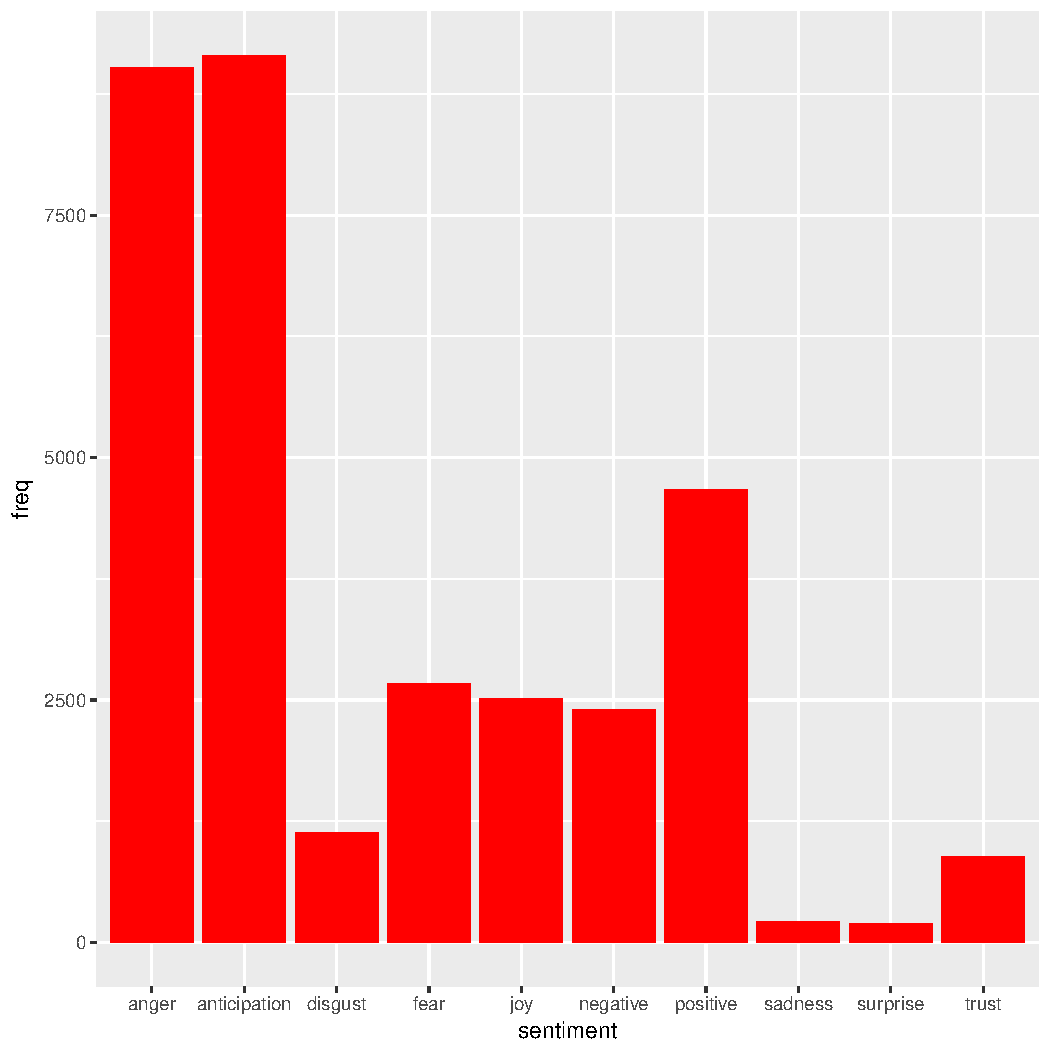
\includegraphics[width=\maxwidth]{figure/unnamed-chunk-5-1} 

\end{knitrout}

\section{wordcloud}

\begin{knitrout}
\definecolor{shadecolor}{rgb}{0.969, 0.969, 0.969}\color{fgcolor}\begin{kframe}
\begin{alltt}
\hlkwd{wordcloud}\hlstd{(two_cities}\hlopt{$}\hlstd{word,two_cities}\hlopt{$}\hlstd{freq,}\hlkwc{min.freq} \hlstd{=}\hlnum{50}\hlstd{,}
          \hlkwc{colors} \hlstd{=} \hlkwd{brewer.pal}\hlstd{(}\hlnum{6}\hlstd{,}\hlstr{'Dark2'}\hlstd{),}\hlkwc{vfont}\hlstd{=}\hlkwd{c}\hlstd{(}\hlstr{"script"}\hlstd{,}\hlstr{"bold"}\hlstd{))}
\end{alltt}
\end{kframe}
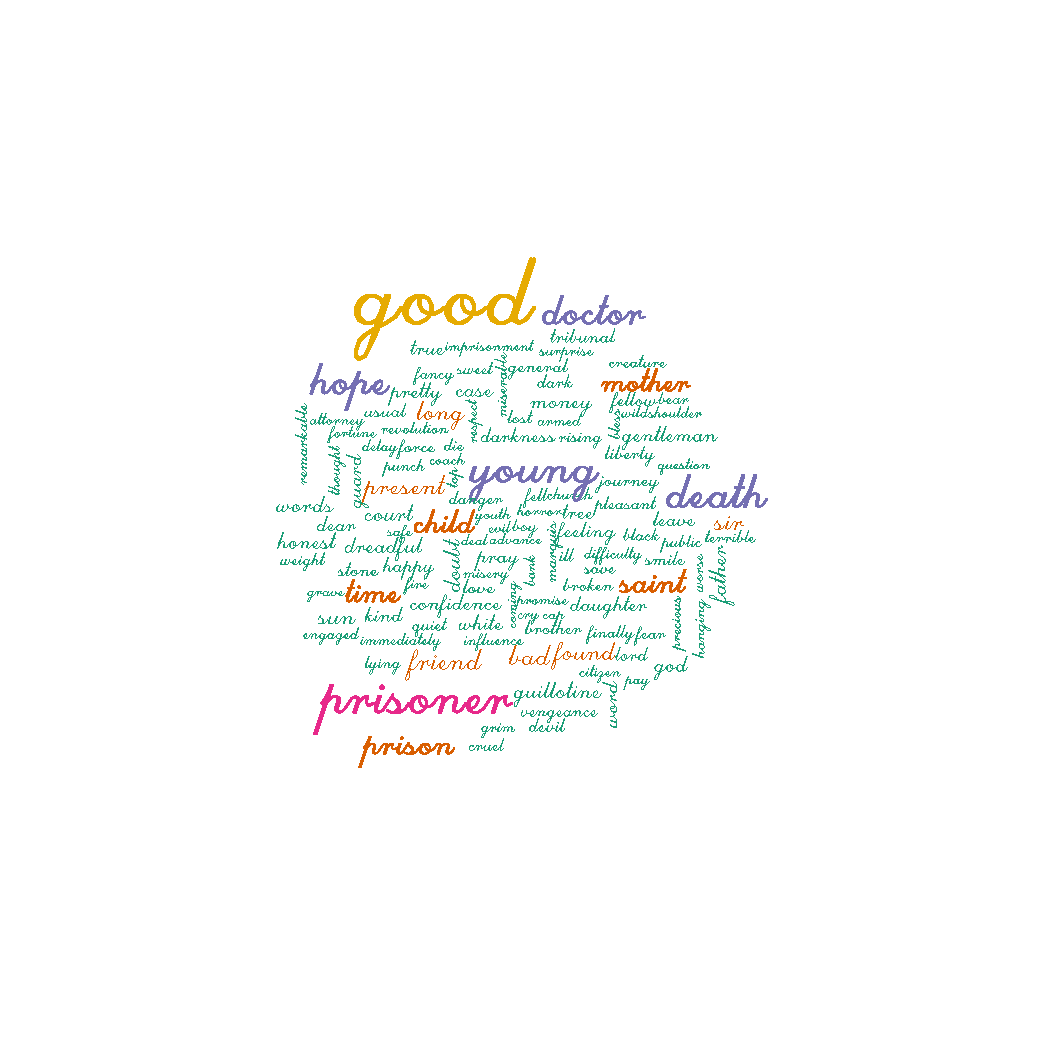
\includegraphics[width=\maxwidth]{figure/unnamed-chunk-6-1} 

\end{knitrout}

\bibliography{CharlesDickens}
\nocite{*}
\end{document}
